\documentclass[twoside]{wfiisul}
%

\usepackage[utf8]{inputenc}
\usepackage{amsmath}
\usepackage{tabularx}
\usepackage[hidelinks]{hyperref}
\usepackage{afterpage}

%\usepackage{pdflscape}
%\usepackage{afterpage}
%\usepackage{changepage}
%\usepackage{caption}
%\usepackage{rotating} %for sidewisetable
%\usepackage{makecell}
%\usepackage{boldline}
%\usepackage{amsthm}
%\usepackage{amsopn}
% włączenie polskich znaków
%\usepackage{lmodern}
%\usepackage{wrapfig}
%\usepackage[table]{xcolor}

\begin{document}

\tytul{Tytuł Pracy Dyplomowej }

\typpracy{inżynierska}

\autor{Imie Nazwisko}
\nralbumu{****}
\kierunek{informatyka}
\specjalnosc{informatyka stosowana}
\specjalizacja{****}

\promotor{***}
\katedra{****}

\stronatytulowa


\chapter{Podział prac na rozdziały}

Poniższy dokument jest przykładowym zastosowaniem szablonu .cls pracy dyplomowej na Wydziale Fizyki i Informatyki Stosowanej UŁ. Każdy rozdział pracy może dzielić się na sekcje i pod-sekcje. Spis treści budowany jest z wykorzystaniem elementów : {\textbackslash}chapter, {\textbackslash}section i {\textbackslash}subsection. Szablon zakłada wydruk dwustronicowy, z tego powodu każdy nowy rozdział rozpoczyna się na stronie nieparzystej.

Praca musi być przygotowana zgodnie z Procedurą dyplomowania przyjętą na Wydziale Fizyki i Informatyki Stosowaniej Uniwersytetu Łódzkiego \cite{Procedura_dyplomowania}.
\section{System \LaTeX}
Można znaleźć wiele źródeł na temat systemu \LaTeX \cite{latex_wiki}.

\chapter{Język pracy}

\section{Spacje i znaki interpunkcyjne}
System latex sam radzi sobie ze wielokrotnymi spacjami, jednakże nie należy ich stosować w tekście. Nowy akapit oznacza się jedną pustą linią w dokumencie .tex. 

Znaki interpunkcyjne takie jak przecinek (,), kropka (.), dwukropek (:), średnik (;), znak zapytania (?), wykrzyknik (!), zamknięcie dowolnego nawiasu (]\})>), zamknięcie cudzysłowu ('' lub ') nie mogą być nigdy poprzedzone spacją. Bezpośrednio po wymienionych znakach może wystąpić wyłącznie spacja, znak nowego akapitu lub inny znak interpunkcyjny. Po znakach otwierających dowolnego nawiasu ([\{(<) lub otwarcia cudzysłowu (`` lub `) nigdy nie należy używać spacji. Spację używamy przed tymi znakami. Nie należy rozpoczynać akapitu od spacji – przerwa ta jest dodawana  automatycznie przez system latex.

Dodatkowo sugeruje się stosowanie twardych spacji w celu unikania wszelkiego rodzaju sierotek, przed ostatecznym wysłaniem pracy do APD należy sprawdzić czy nie występują  bękarty, sierotki, wdowy i szewcy \cite{Bekart}.

\section{Wzory matematyczne}
W systemie latex występują dwa główne rodzaje wzorów, wstawiane w element zdania $E = mc^2$, tworzone za pomocą środowiska \$\dots\$, jak i umieszczane w osobnych linijkach z wykorzystaniem środowisk: \textit{equation, equation* (\textbackslash[\dots\textbackslash])}
\begin{equation}\label{eq:wn}
W(n) = \bigotimes_{n} W(1),
\end{equation}
where:
\begin{equation}\label{eq:w1}
W(1) = \begin{bmatrix}
         1 & 1 \\
         1 & -1 \\
       \end{bmatrix}.
\end{equation}

Należy pamiętać iż do numerowanych wzorów odnosimy się za pomocą środowisk {\textbackslash}label i {\textbackslash}eqref. Dla przykładu wzór \eqref{eq:wn} opisuje wielowymiarową transformatę Walsha z wykorzystaniem transformaty jednowymiarowej \eqref{eq:wn}.

\subsection{Skomplikowane wzory matematyczne}
W celu uzyskania bardziej skomplikowanych wzorów, np łamania wzorów wieloliniowych zaleca sie wykorzystanie biblioteki \textit{amsmath} a w szczególności \textit{align, gather, multline, \dots}, bardziej szczegółowe opisy można znaleźć w \cite{latex_math_wiki}.

\section{Elementy pływające}
Każdy element pływający jak: obrazek, schemat, tabela czy fragment z~kodem źródłowym powinien zostać odpowiednio oznaczony (ponumerowany) i~zatytułowany. W~pracy powinno znaleźć się co najmniej jedno odwołanie do wspomnianego elementu, w~innym wypadku sprawia to wrażenie, iż element jest zbędny. Przykładowe odniesienie do obrazków oraz tabel oznaczamy za pomocą {\textbackslash}ref, dla przykładu na Rysunku \ref{diagram_wybranej_klasy} przedstawiono diagram klasy a Tabela \ref{rest1} zawiera opis elementu API typu REST. Dodatkowo należy pamiętać, iż zasady umieszczania elementów pływających w~tekście ograniczają znacząco jaką część strony mogą zawierać, a~co za tym idzie omawiana tabelka, obrazek nie muszą znajdować się w~bezpośrednim sąsiedztwie tekstu odnoszącego się do obiektu.

\begin{figure}[!h]
\centering
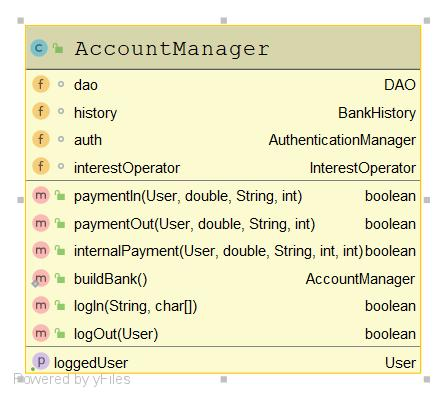
\includegraphics[width = 200pt]{DiagramKlasy.jpg}
\caption{Przykładowy diagram opisujący jedną klasę.}\label{diagram_wybranej_klasy}
\end{figure}

\begin{table}
\begin{tabularx}{\textwidth}{|l|X|}
\hline
&\textbf{Pobranie wybranego rekordu}\\\hline
URL &   \url{http://geniusgamedev.eu/cordova/rest_api/rest_srv/:id} lub \url{http://geniusgamedev.eu/cordova/rest_api/rest.php?id=:id}\\\hline
Method  & GET\\\hline
Parameters  & id - id wybranego elementu \\\hline
Request Data & None\\\hline
Response Data & obiekt w postaci:\\
&

%\begin{js}
\{'data':\{
    'id':2,
    'name':'Helena',
    'score':128
    \}
\}
%\end{js}

\\\hline
\end{tabularx}
\caption{Metoda get stosowanej usługi REST}\label{rest1}
\end{table}

\section{Cytowania}
Cytowania należy oznaczać wykorzystując {\textbackslash}cite. Wielokrotne cytowania należy grupować \cite{Bekart, Cytowanie, latex_math_wiki, Procedura_dyplomowania} W pracy należy stosować jeden z trzech systemów cytowań (Vancouver System, Harvard System, Oxford System) opisanych szczegółowo w \cite{Cytowanie}, regulamin dyplomowania zaleca wykorzystanie systemu \underline{Vancouver}. W~przypadku systemów Vancouver i Oxford bibliografia powinna być posortowana w kolejności pojawiania się odwołań w tekście, natomiast w systemie Harvard alfabetycznie wedle nazwisk pierwszych autorów.

\clearpage
\tableofcontents
%\listoftables
%\listoffigures

\thebibliography{99}
\bibitem{Procedura_dyplomowania} Procedura dyplomowania na WFiIS UŁ:
\url{http://wfi.uni.lodz.pl/student/procedury-akty-prawne-i-formularze/#toggle-id-1}
\bibitem{latex_wiki} Wiki page about LaTeX: \url{https://en.wikibooks.org/wiki/LaTeX}.

\bibitem{Bekart} Strony Wikipedii poświęcone błędom w łamaniu tekstu\\
\url{https://pl.wikipedia.org/wiki/B%C4%99kart_(typografia)}

\bibitem{latex_math_wiki} Wiki page about LaTeX/Advanced Mathematics: \url{https://en.wikibooks.org/wiki/LaTeX/Advanced_Mathematics}.

\bibitem{Cytowanie} Strona Wikipedii poświęcona metodom cytowania \\
\url{https://pl.wikipedia.org/wiki/Cytowanie_pi%C5%9Bmiennictwa}

\end{document}
